\documentclass[a4paper,12pt]{report}
\usepackage{cmap} % поиск в пдф
\usepackage[T2A]{fontenc} % кодировка
\usepackage[utf8]{inputenc} % кодировака исходного текста
\usepackage[english, russian]{babel} % локализация и переносы
\usepackage{amsmath}
\usepackage{graphicx}
\graphicspath{./}
\documentclass[main.tex]{subfiles}


\begin{document}
	
	\begin{center}
		\section*{Тест на дальтонизм}
	\end{center}

	Тест был разработан на основе исследований ученых, работающих в самых лучших научных лабораториях мира. На данный момент, этот тест самый инновационный в плане выявления дальтонизма у больных людей. 
	
	Производится следующая градация уровней дальтонизма:
	\begin{itemize}
		\item Протанопия - при которой человек не отличает зеленые оттенки от красных;
		\item Дейтеранопия - больной человек не отличиет зеленый цвет от синего;
		\item Тританопия - нарушение зрения в сине-фиолетовой части спектра. Человек видит только красные и зеленые оттенки;
		\item Трихромазия - человек различает три основных цвета. При этом это состояние может быть вполне нормальным и не характеризоваться как дальтонизм.
		\item Ахроматопсия - характеризуется полным отсутствием цветовых ощущений.
	\end{itemize}

	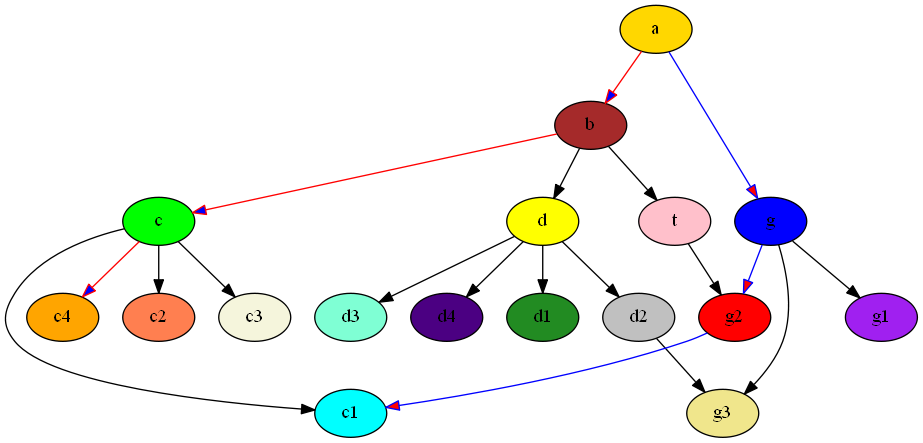
\includegraphics[scale=0.45]{ex2.png}


	Если вы можете различить все цвета на этой картинке, значит вы здоровы! (но это не точно)
\end{document}